%%%%%%%%%%%%%%%%%%%%%%%%%%%%%%%%%%%%%%%%%
% Beamer Presentation
% LaTeX Template
% Version 1.0 (10/11/12)
%
% This template has been downloaded from:
% http://www.LaTeXTemplates.com
%
% License:
% CC BY-NC-SA 3.0 (http://creativecommons.org/licenses/by-nc-sa/3.0/)
%
%%%%%%%%%%%%%%%%%%%%%%%%%%%%%%%%%%%%%%%%%

%----------------------------------------------------------------------------------------
%	PACKAGES AND THEMES
%----------------------------------------------------------------------------------------

\documentclass{beamer}

\mode<presentation> {

% The Beamer class comes with a number of default slide themes
% which change the colors and layouts of slides. Below this is a list
% of all the themes, uncomment each in turn to see what they look like.

%\usetheme{default}
%\usetheme{AnnArbor}
%\usetheme{Antibes}
%\usetheme{Bergen}
%\usetheme{Berkeley}
%\usetheme{Berlin}
%\usetheme{Boadilla}
\usetheme{CambridgeUS}
%\usetheme{Copenhagen}
%\usetheme{Darmstadt}
%\usetheme{Dresden}
%\usetheme{Frankfurt}
%\usetheme{Goettingen}
%\usetheme{Hannover}
%\usetheme{Ilmenau}
%\usetheme{JuanLesPins}
%\usetheme{Luebeck}
%\usetheme{Madrid}
%\usetheme{Malmoe}
%\usetheme{Marburg}
%\usetheme{Montpellier}
%\usetheme{PaloAlto}
%\usetheme{Pittsburgh}
%\usetheme{Rochester}
%\usetheme{Singapore}
%\usetheme{Szeged}
%\usetheme{Warsaw}

% As well as themes, the Beamer class has a number of color themes
% for any slide theme. Uncomment each of these in turn to see how it
% changes the colors of your current slide theme.

%\usecolortheme{albatross}
%\usecolortheme{beaver}
%\usecolortheme{beetle}
%\usecolortheme{crane}
%\usecolortheme{dolphin}
%\usecolortheme{dove}
%\usecolortheme{fly}
%\usecolortheme{lily}
%\usecolortheme{orchid}
%\usecolortheme{rose}
%\usecolortheme{seagull}
\usecolortheme{seahorse}
%\usecolortheme{whale}
%\usecolortheme{wolverine}

\setbeamertemplate{footline} % To remove the footer line in all slides uncomment this line
%\setbeamertemplate{footline}[page number] % To replace the footer line in all slides with a simple slide count uncomment this line

%\setbeamertemplate{navigation symbols}{} % To remove the navigation symbols from the bottom of all slides uncomment this line
}

\usepackage{graphicx} % Allows including images
\usepackage{booktabs} % Allows the use of \toprule, \midrule and \bottomrule in tables

% add for formula and theorems
\usepackage{amsthm}  % added again for properly using thmtools, seems i overwrite sth..
\usepackage{amssymb} % for symbols
\usepackage{multirow} % for table
\usepackage{mathrsfs} % for fancy characters like z-transform
\usepackage{thmtools}
\usepackage{array} % for customize the distance between columns in a array
%\declaretheoremstyle[headfont=\scshape,postheadspace=\newline]{mystyle}
%\declaretheorem[style=mystyle]{theorem}
%\newcounter{mytempeqncnt}

\usepackage{blkarray} % Used for multi-blocks matrix
%\usepackage{easybmat}

%\newtheorem{theory}{Theorem}
%\newtheorem{lemma}{Lemma}
%\newtheorem{corollary}{Corollary}
%\newtheorem{property}{Property}
%\newtheorem{define}{Definition}
%\newtheorem{remark}{Remark}
%\usepackage{bbm}
%\usepackage[justification=centering]{caption}
%\usepackage{ctable} % for \specialrule command
\usepackage{mathtools} % for \coloneqq




%----------------------------------------------------------------------------------------
%	TITLE PAGE
%----------------------------------------------------------------------------------------

\title[Capacity Analysis of Coprime Communication]{Capacity Analysis of Coprime Communication} % The short title appears at the bottom of every slide, the full title is only on the title page

\author{Qiong Wu} % Your name
\institute[UCLA] % Your institution as it will appear on the bottom of every slide, may be shorthand to save space
{
University of Texas at Arlington \\ % Your institution for the title page
Wireless Comm. and Networking Lab\\
\medskip
\textit{qiong.wu@mavs.uta.edu} % Your email address
}
\date{\today} % Date, can be changed to a custom date

\begin{document}

\begin{frame}
\titlepage % Print the title page as the first slide
\end{frame}

\begin{frame}
\frametitle{Overview} % Table of contents slide, comment this block out to remove it
\tableofcontents % Throughout your presentation, if you choose to use \section{} and \subsection{} commands, these will automatically be printed on this slide as an overview of your presentation
\end{frame}

%----------------------------------------------------------------------------------------
%	PRESENTATION SLIDES
%----------------------------------------------------------------------------------------

%------------------------------------------------
\section{Introduction} % Sections can be created in order to organize your presentation into discrete blocks, all sections and subsections are automatically printed in the table of contents as an overview of the talk
%------------------------------------------------

%\subsection{Subsection Example} % A subsection can be created just before a set of slides with a common theme to further break down your presentation into chunks


\begin{frame}
\frametitle{Introduction}
The study of capacity of analog Gaussian channels and capacity-achieving transmission strategies was pioneered by Shannon, whose work focused on capacity of channels sampled at or above twice the channel bandwidth.\\~\\

However, in practice, the Nyquist rate may be {\bf excessive} for perfect reconstruction of signals that the transmission channel possess certain structures known a priori. On the other hand, the {\bf hardware} and {\bf power limitations} may preclude sampling at the Nyquist rate for a wideband communication system.\\~\\

This motivates the exploration of the effects of sub-Nyquist sampling upon the capacity of an analog Gaussian channel, and the capacity limits that result from general sampling methods.
\end{frame}

\begin{frame}
\frametitle{Related works}
\begin{itemize}
  \item When the channel or signal structure is unknown, the blind sub-Nyquist sampling approaches have be proposed to exploit the structure of various classes of input signals based on sampling with modulation and filter banks [Mishali, 2010].
  \item At the transmitter side, although MRC maximizes the combiner SNR for a MISO channel, it is suboptimal for the joint optimization problem compared with selection combining [Goldsmith, 2005].
  \item The capacity with sampling rate under filter-banks with/without modulation are not monotonously increasing, which indicates that more sophisticated sampling techniques are necessary to maximize the capacity  [Chen, 2013].

\end{itemize}
\end{frame}

%------------------------------------------------

\section{Preliminaries}

\begin{frame}
\frametitle{Preliminaries: Revisit Coprime}
\begin{columns}[c] % The "c" option specifies centered vertical alignment while the "t" option is used for top vertical alignment

\column{.5\textwidth} % Left column and width
\begin{figure}
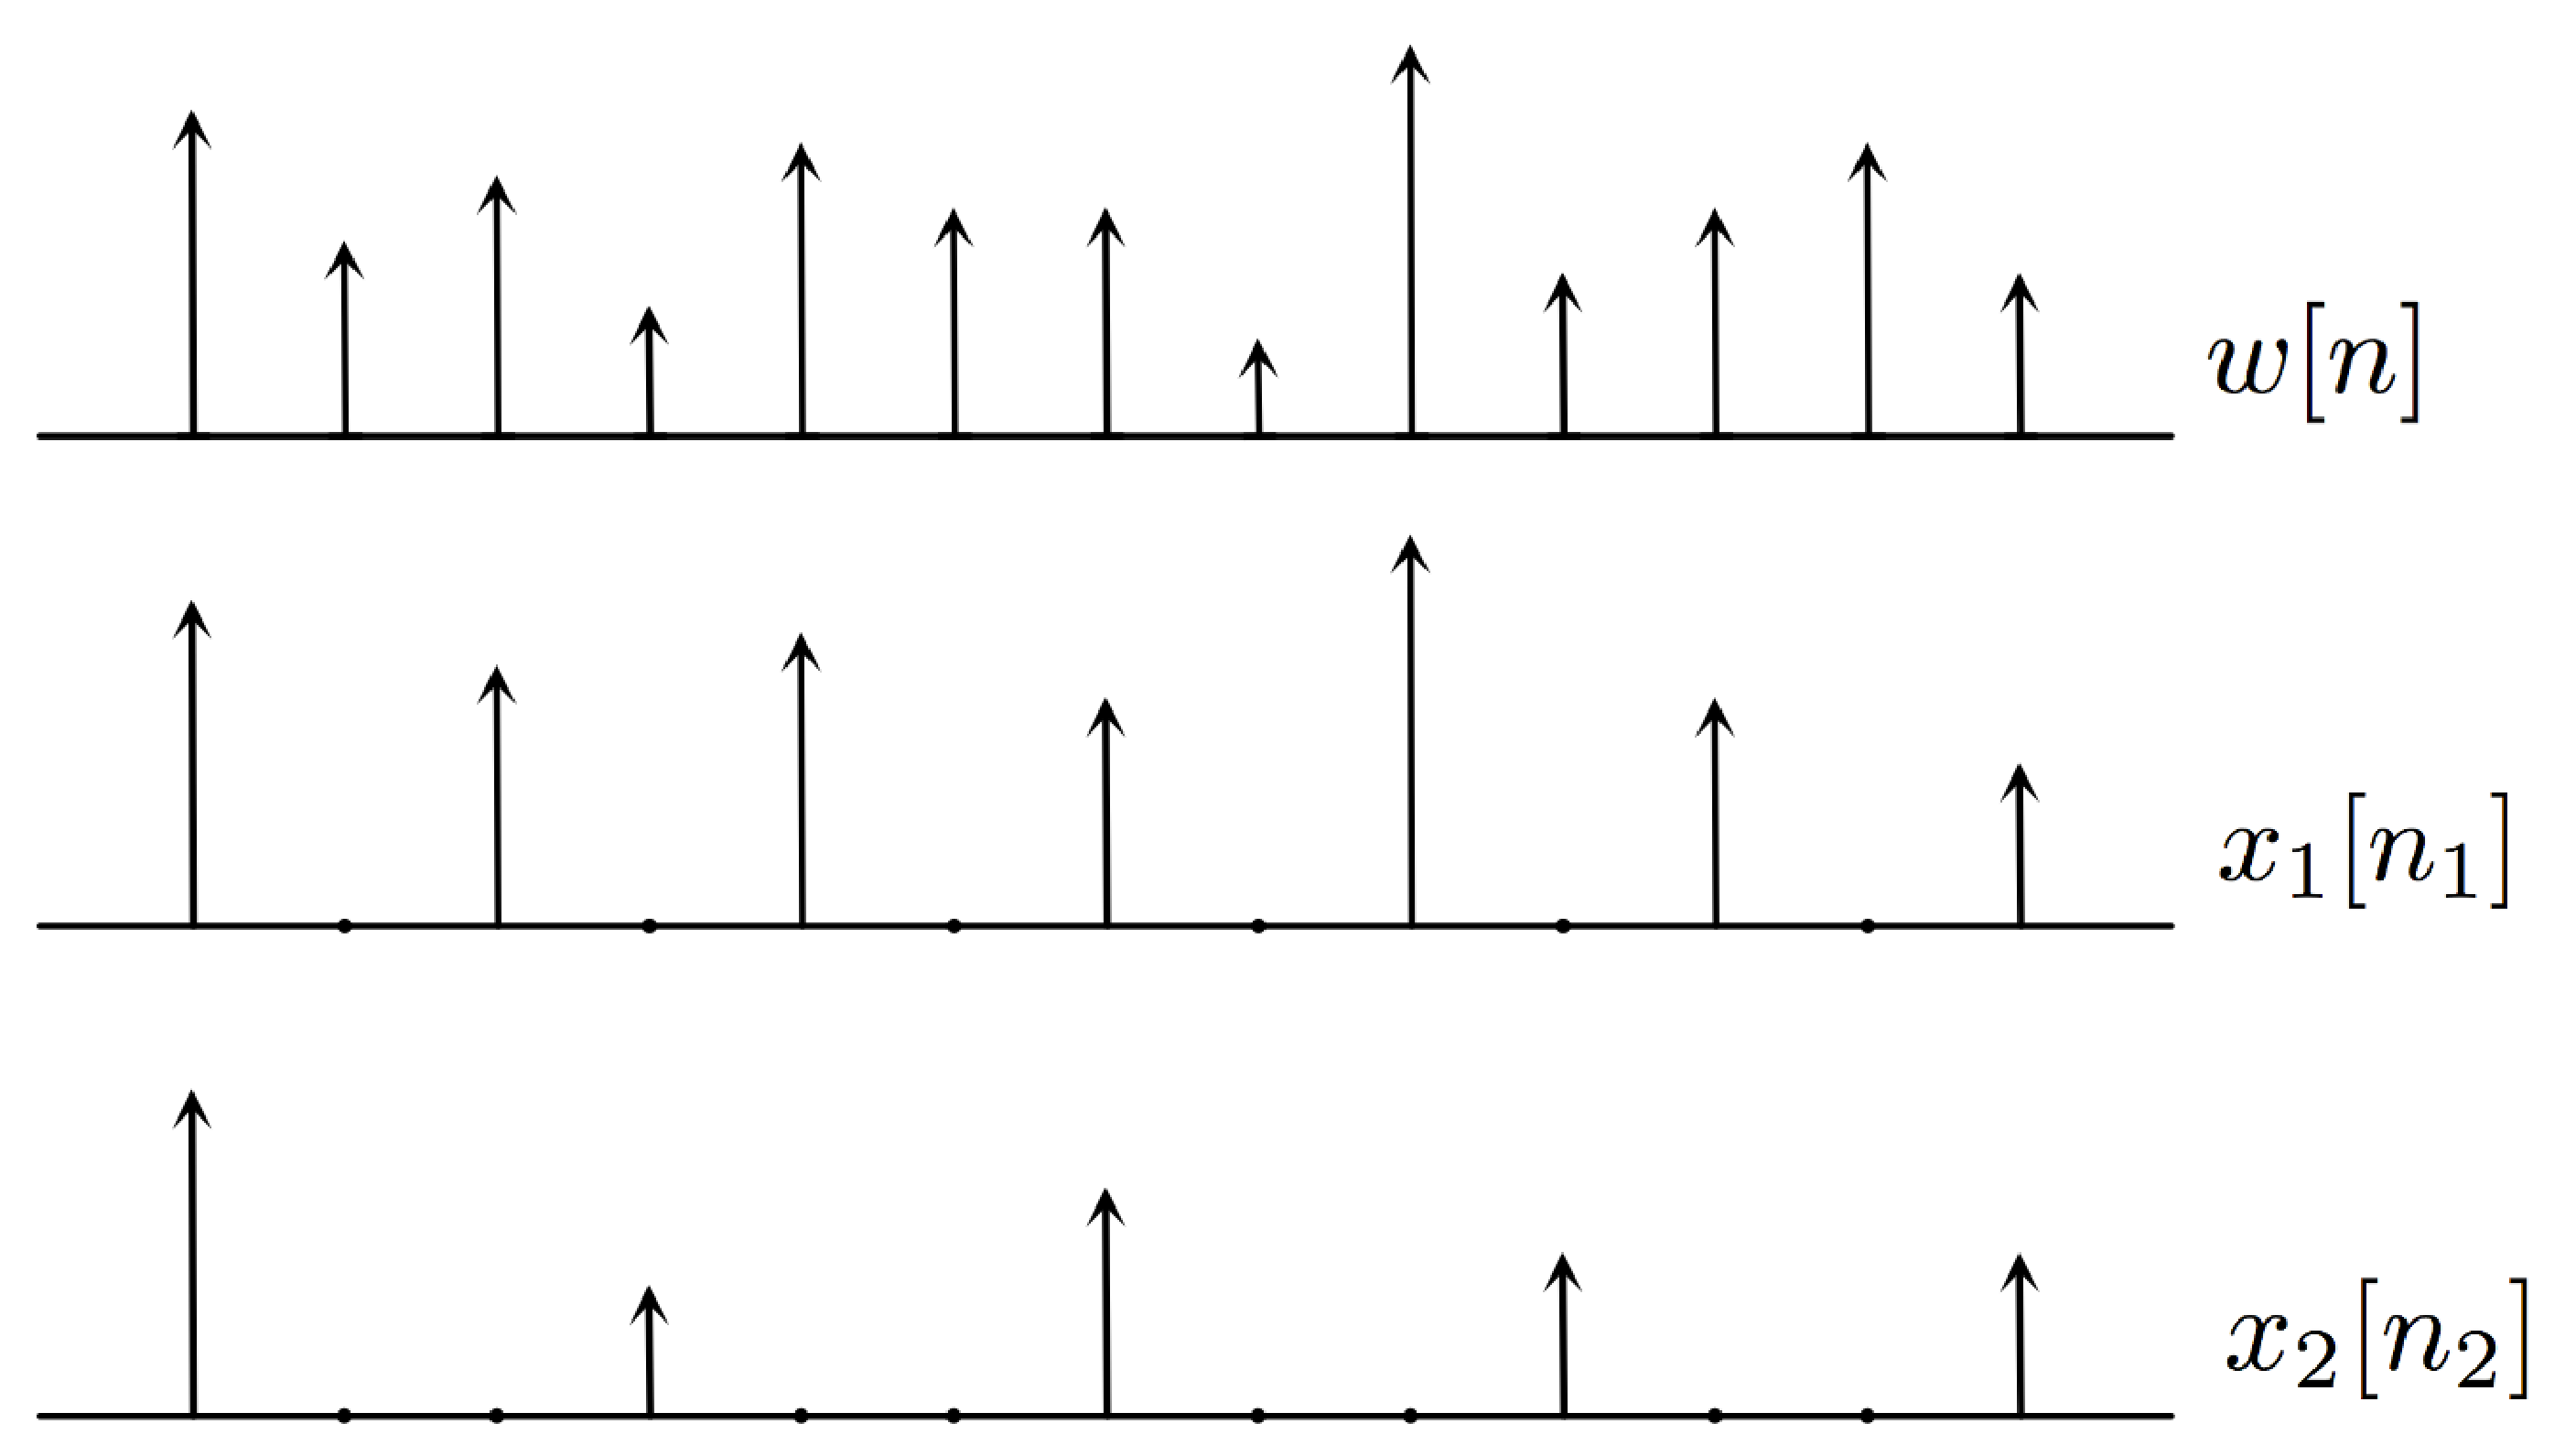
\includegraphics[width=1\linewidth]{illustrate.pdf}
\end{figure}

\column{.5\textwidth} % Right column and width
\begin{figure}
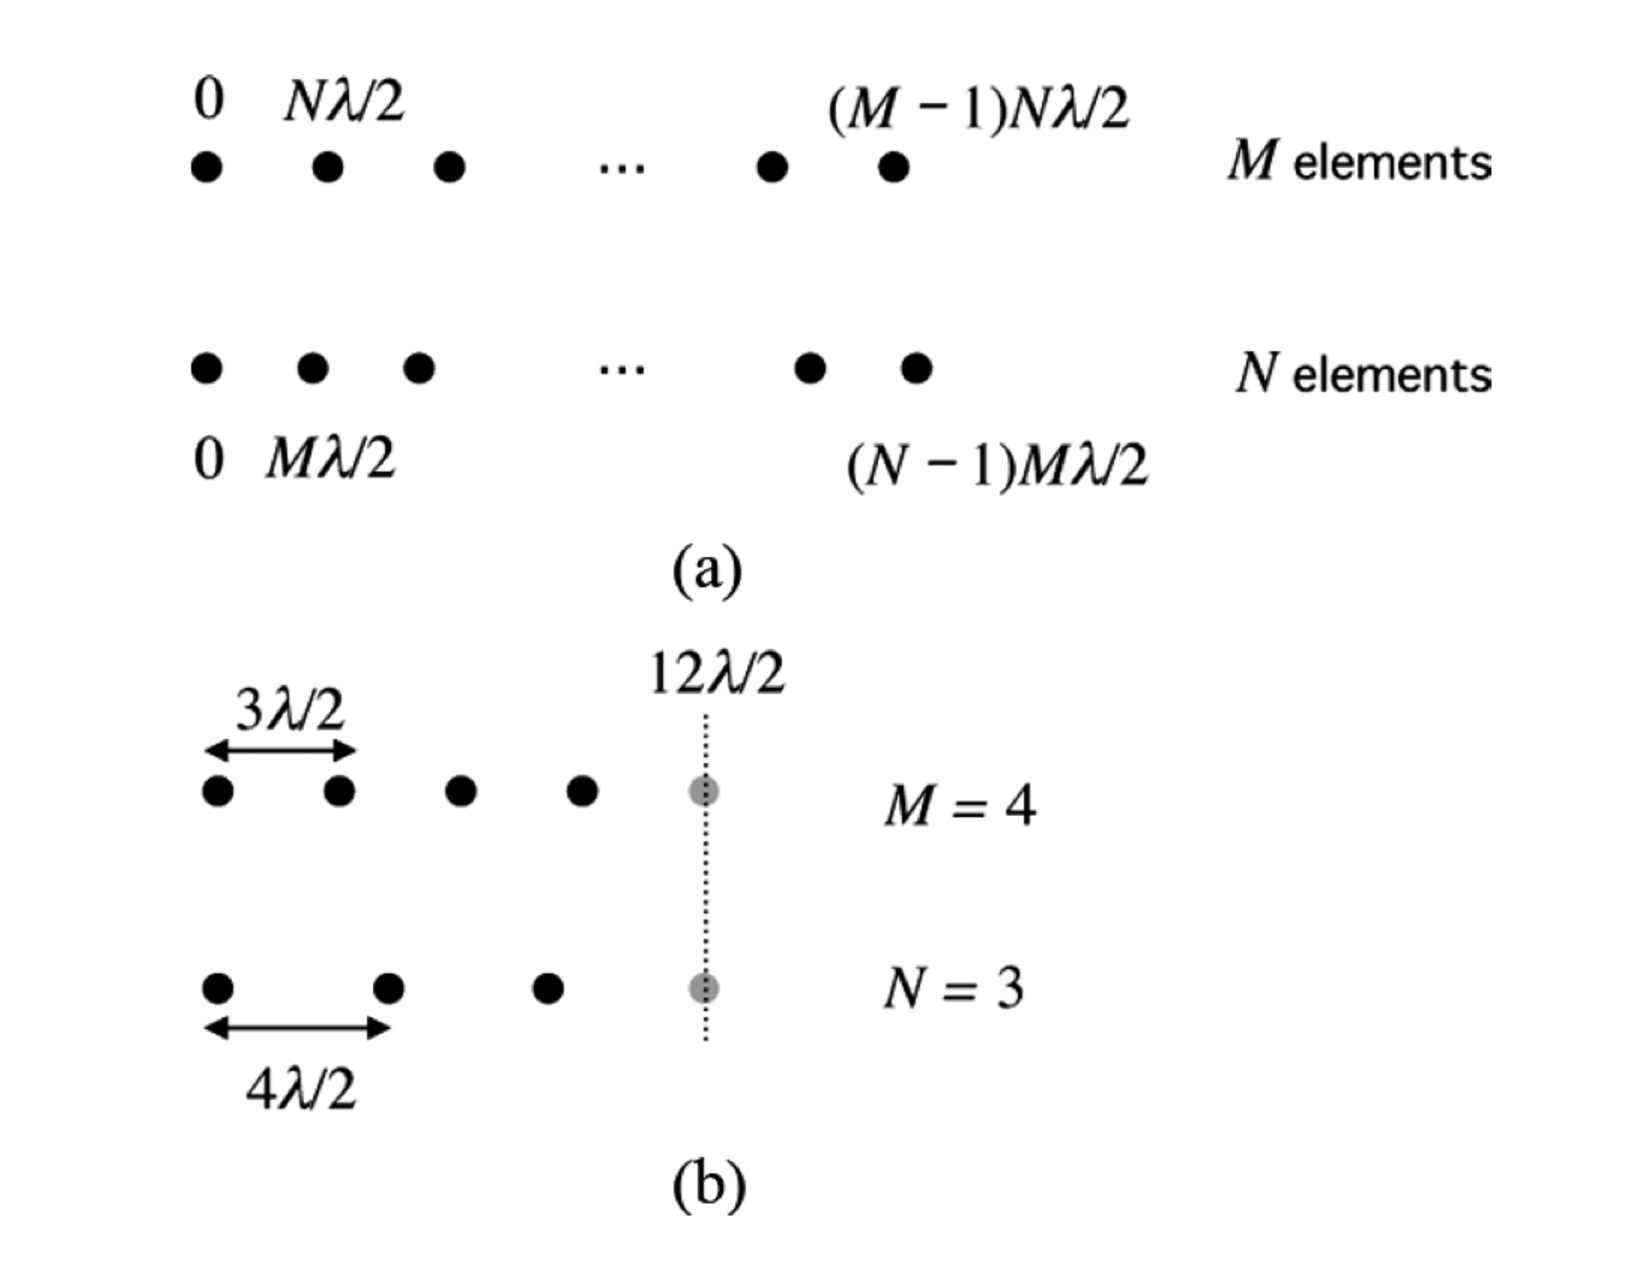
\includegraphics[width=1\linewidth]{coprime_sampling.pdf}
\end{figure}

\end{columns}
\end{frame}

\begin{frame}
\frametitle{Theorem 1: Channel capacity}
\begin{block}{}
  \cite[Th. 8.5.1]{Gallager:1968} For the channel with a power constraint $P$ and noise PSD $N(f)$, assume that $|H(f)|^2/N(f)$ is bounded and integrable, and that either $\int\limits_{-\infty}^{+\infty}N(f)df<+\infty$ or that $N(f)$ is white. Then the channel capacity is given by
  \begin{equation}
    \label{nyquist_rate}
    \mathbb{C}=\frac{1}{2}\int\limits_{-\infty}^{+\infty}\log^+\left( \nu\frac{|H(f)|^2}{N(f)}\right)df,
  \end{equation}
where $\nu$ is the water-filling for additive Gaussian channel and satisfying
\begin{equation}
  \int\limits_{-\infty}^{+\infty}\left[\nu-\frac{N(f)}{|H(f)|^2}\right]^+df=P.
\end{equation}
\end{block}
\end{frame}

\begin{frame}
\frametitle{Theorem 2: Landau Sampling Rate}
\begin{block}{}
  \cite[Th. 1 and Lemma 4]{Landau:1967} Given a fixed set $S$ of N-frequency bands whose total finite length, including both the negative and positive frequencies, denoted by $m(S)$, the space $\mathscr{B}(S)$ of all signals of finite energy with frequencies contained only in $S$, and $\Lambda$ is a sampling set from $\mathscr{B}(S)$, All signals $f(t)\in\mathscr{B}(S)$ can be uniquely determined by their samples $\{f(t_n)|t_n\in\Lambda\}$ only if the lower Beurling density $D^-(\Lambda)$ satisfying
  \begin{align}
    D^-(\Lambda) &= \lim_{r\to\infty}\inf\frac{n^-(r)}{r} \nonumber \\
    & \geq \lim_{r\to\infty}\left[\frac{m(S)}{2\pi}-\frac{A\log^+(r)-B}{r}\right]
   \end{align}
with constant $A$ and $B$ relevant with the choices of $S$ and $\Lambda$ and independent of the sampling interval $r$.
\end{block}
\end{frame}

\begin{frame}
\frametitle{Basics of Toeplitz Matrix}
\begin{equation}
   T_n = \begin{bmatrix}
     t_0 & t_{-1} & t_{-2} & \dots & t_{-(n-1)} \\
     t_1 & t_0 & t{-1} & \dots & t_{-(n-2)} \\
     t_2 & t_1 & t_0 & \dots & t_{-(n-3)} \\
     \vdots & \vdots& \vdots & \ddots & \vdots \\
     t_{n-1} & t_{n-2} & t_{n-3} & \dots & t_0 \\
     \end{bmatrix}
\end{equation}
\begin{itemize}
  \item Toeplitz matrices are closely related with Fourier series, and has the property of asymptotical commutation.
  \item A Toeplitz matrix can be briefly described as $T_n=[t_{i-j};i,j=0,1,\dots,n-1]$, which is uniquely defined by the sequence $\{t_k\}$.
\end{itemize}
\end{frame}

\begin{frame}
\frametitle{Basics of Toeplitz Matrix}
The $n\times n$ Toeplitz matrix generated by Fourier coefficients is
\begin{equation}
  T_n(f)=\left[\int_0^{2\pi}f(\lambda)e^{j(i-k)\lambda}\frac{d\lambda}{2\pi};\quad k,i=0,1,\dots,n-1\right].
\end{equation}
Besides, let $U_n$ be the circulant matrix of $T_n$ by filling in the upper right and lower left corners with the appropriate entries. In particular, $U_n$ consists of cyclic shifts of $[c_0^{(n)},\dots,c_{n-1}^{(n)}]$ where
  \begin{equation}
    c_k^{(n)}=\left\{ 
      \begin{array}{l l}
        t_{-k} & \quad k=0,1,\dots,m \\
        t_{n-k} & \quad k=n-m,\dots,n-1. \\
        0 & \quad \text{otherwise} \\
      \end{array} \right.
  \end{equation}
Similarly, the Fourier coefficients of the circulant matrix $U_n(f)$ is also well defined
\begin{equation}
  \label{fourier_circulant}
  U_n(f) = \left[\frac{1}{n}\sum_{j=0}^{n-1}f\left(\frac{2\pi j}{n}\right)e^{\left(\frac{2\pi ijk}{n}\right)};i,k=0,1,\dots,n-1\right].
\end{equation}

\end{frame}


\begin{frame}
\frametitle{Definition: Asymptotic Equivalence of Toeplitz Matrix}
\begin{block}{}
\cite{Gray:2006} Two $n\times n$ matrices $\{A_n\}$ and $\{B_n\}$ are said to be asymptotically equivalent and be abbreviated as $A_n\sim B_n$ if
  \begin{itemize}
    \item $A_n$ and $B_n$ are uniformly bounded for any integer $n$ and a constant $\Psi$ independent of $n$:
      \begin{equation}
        ||A_n||_2, ||B_n||_2\leq\Psi<+\infty
      \end{equation}
    \item The determinant of the differnece between $A_n$ and $B_n$ is approximately zero as $n\to\infty$.
      \begin{equation}
        \lim_{n\to\infty}|A_n-B_n|=0
      \end{equation}
  \end{itemize}
\end{block}
\end{frame}

\begin{frame}
\frametitle{Lemma 1: Eighenvalues of Toeplitz Matrices}
\begin{block}{}
  \cite[Lemma 1]{Gray:2006} Suppose $A_n\sim B_n$ with eighenvalues $\{\alpha_{n,k}\}$ and $\{\beta_{n,k}\}$, respectively. Let $g(x)$ be an arbitrary continuous function. Then,
  \begin{equation}
    \lim_{n\to\infty}\frac{1}{n}\sum_{k=0}^{n-1}g(\alpha_{n,k}-\beta_{n,k})=0
  \end{equation}
  and hence if either limit exists individually,
  \begin{equation}
    \lim_{n\to\infty}\frac{1}{n}\sum_{k=0}^{n-1}g(\alpha_{n,k})=\lim_{n\to\infty}\frac{1}{n}\sum_{k=0}^{n-1}g(\beta_{n,k})
  \end{equation}
\end{block}
\end{frame}

\begin{frame}
\frametitle{Lemma 2: Operations of Toeplitz Matrices}
\begin{block}{}
  \cite[Lemma 7 and 10]{Gray:2006}
  \label{lemma2}
  \begin{itemize}
    \item Suppose a banded Toeplitz matrix $T_n=\{t_{i-j};i,j=0,1,\dots,n-1\}$, which satisfies that $\{t_k\}$ is absolutely summable, and the Fourier serieris $f(\lambda)$ related to $T_n$ is positive and $T_n$ is Hermitian.
  Then we have
  \begin{equation}
    T_n(f)\sim U_n(f)
  \end{equation}
  If $f(\lambda)$ is real and there exists a constant $\varepsilon>0$ such that $\inf{f}\geq\varepsilon$, then
  \begin{equation}
    T_n(f)^{-1}\sim U_n(f)^{-1}=U_n(1/f)\sim T_n(1/f)
  \end{equation}
\item Suppose $\pmb{A}_n\sim\pmb{B}_n$ and $\pmb{C}_n\sim\pmb{D}_n$, then $\pmb{A}_n\pmb{C}_n\sim\pmb{B}_n\pmb{D}_n$.
  \end{itemize}
\end{block}
\end{frame}

%------------------------------------------------


\section{System Modeling}

\begin{frame}
\frametitle{System Modeling}
\begin{figure}
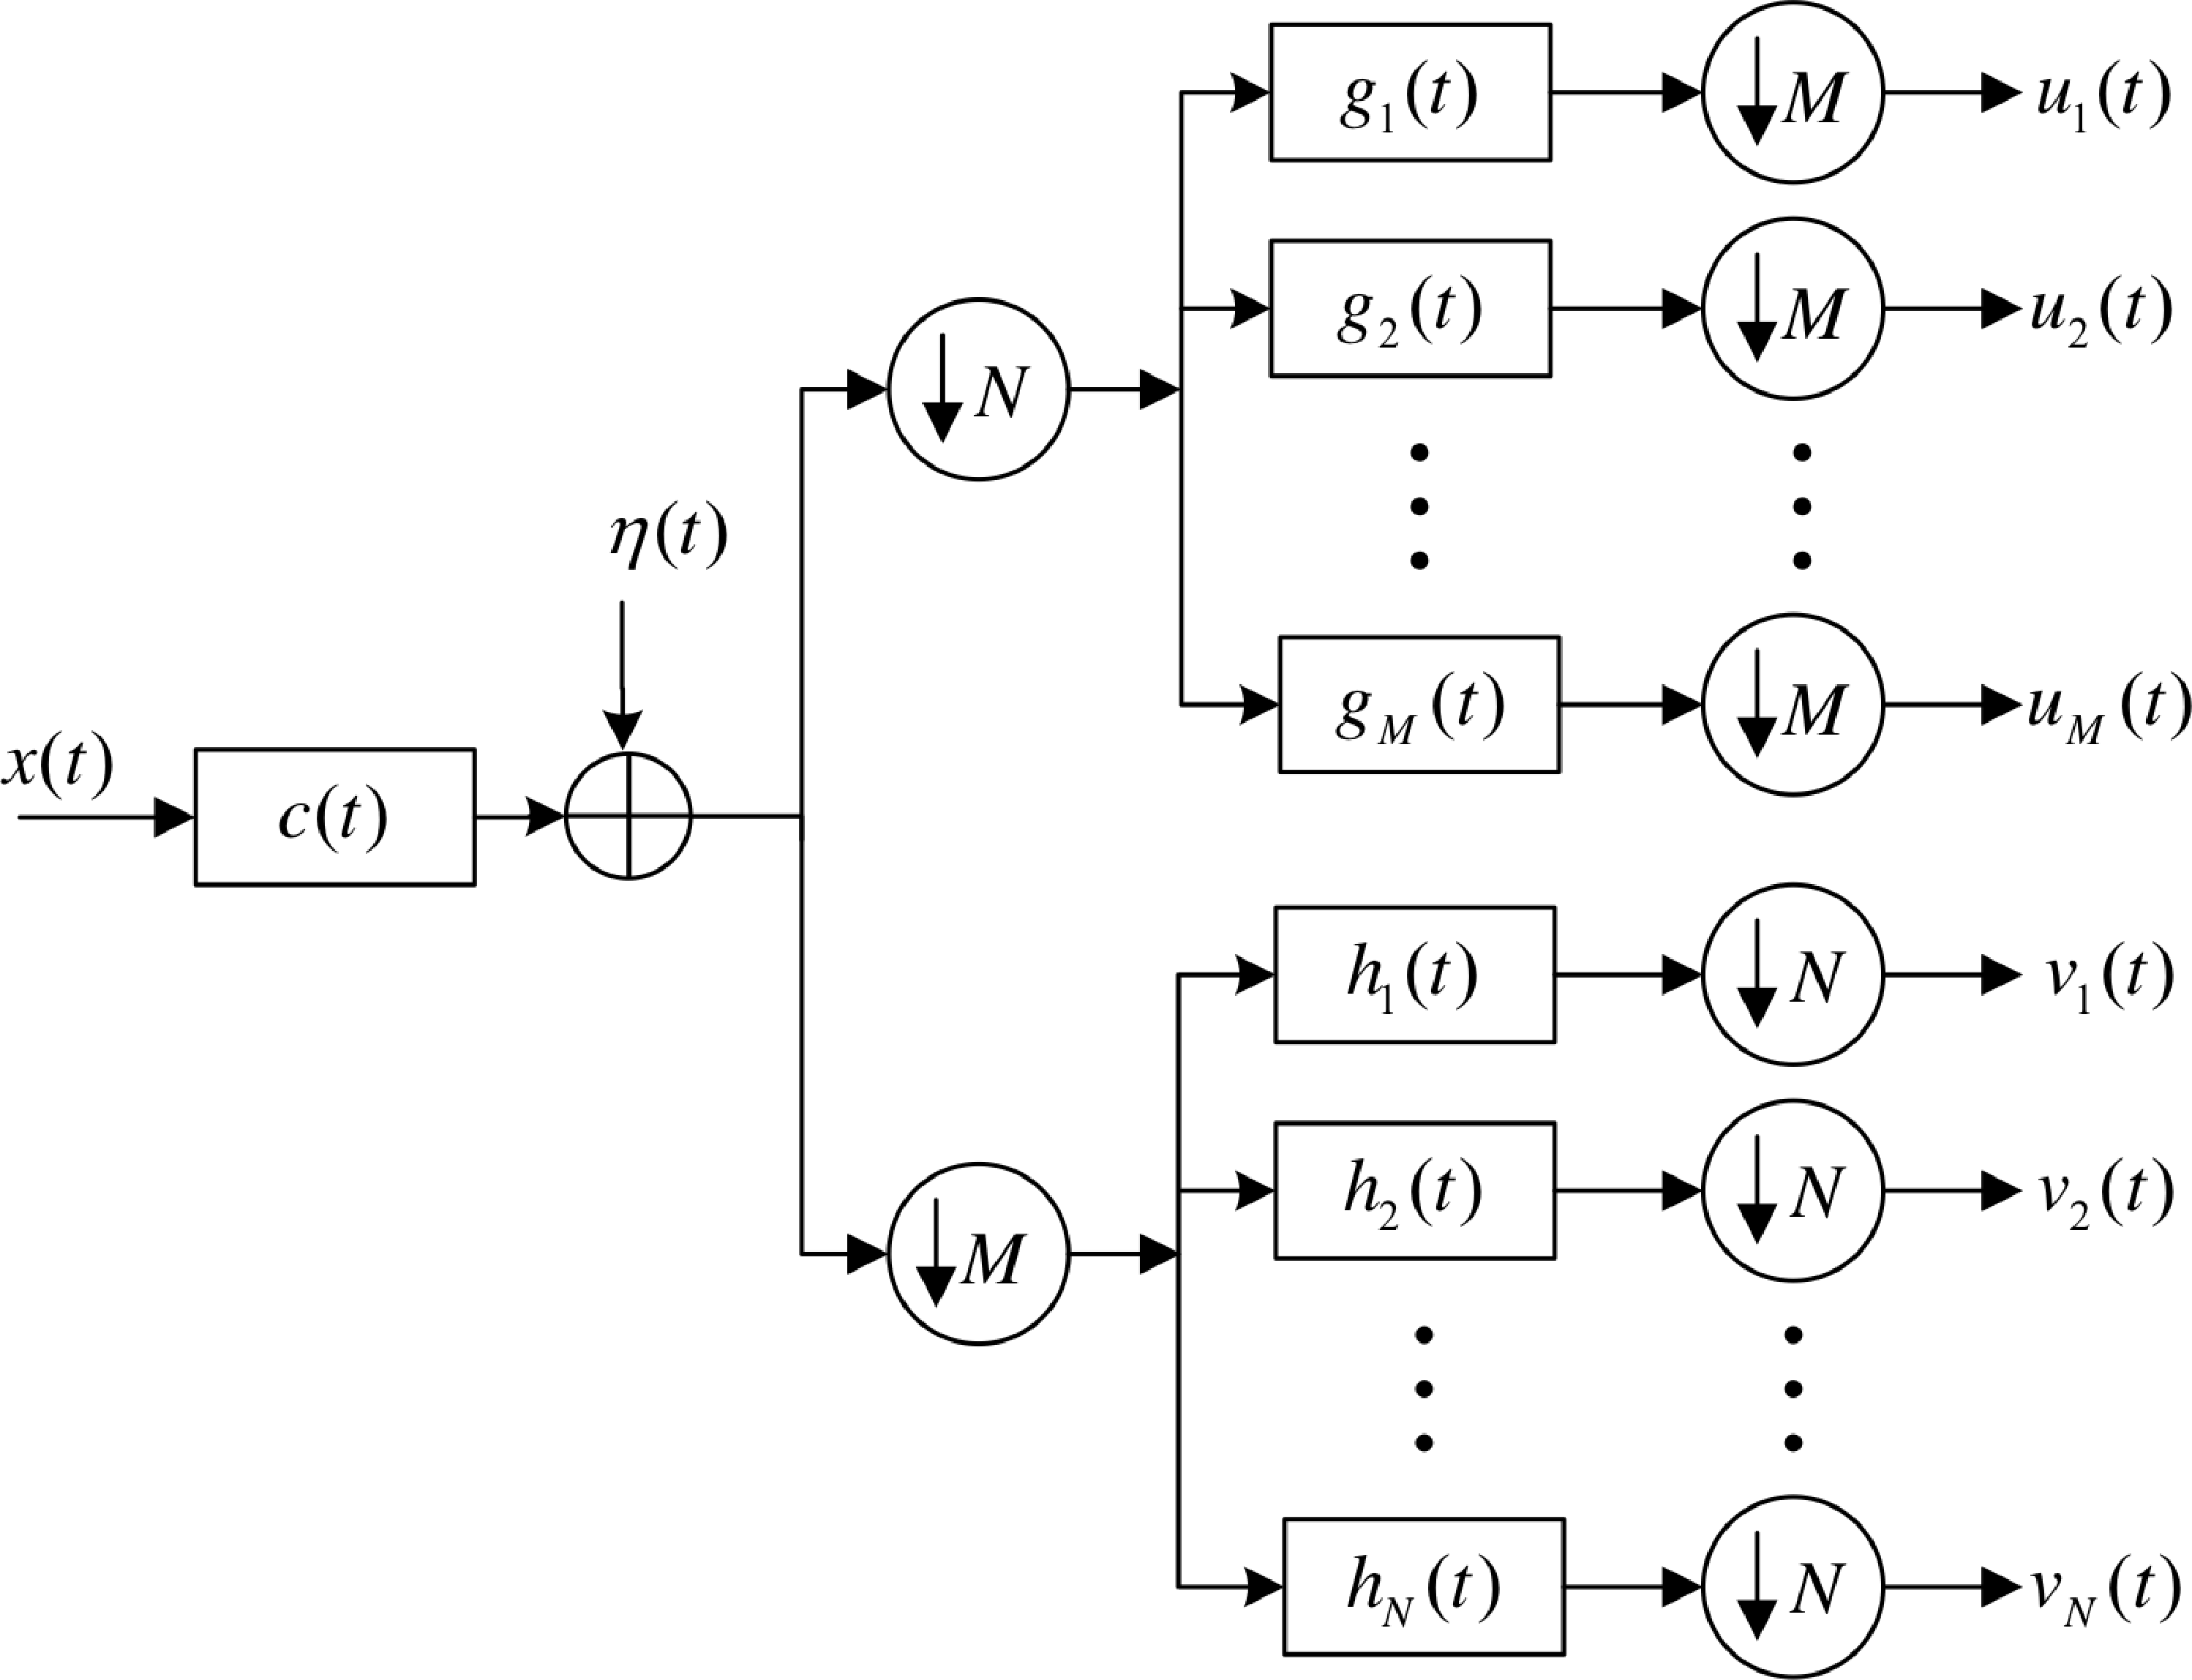
\includegraphics[width=0.7\linewidth]{flowchart1.pdf}
\end{figure}
\end{frame}

\begin{frame}
\frametitle{Matrices of Impulse Responses}
\begin{align}
  \pmb{G}_m &=[\dots\text{ }G_{m,-1}\text{ }G_{m,0}\text{ }G_{m,1}\text{ }\dots]\quad 1\leq m\leq M \\
  G_{m,0} &=[g^0_m,\underbrace{0,\dots,0}_\text{N-1},g^N_m,0,\dots,0,g^{\frac{L-1}{M}}_m]^T
\end{align}
\begin{equation}
    \pmb{G}_m = \begin{bmatrix}
      \dots & g_m^0 & 0 & \dots & 0 & g_m^{-N} & \dots \\%[1.5mm]
      \dots & 0 & g_m^0 & \dots & 0 & 0 & \dots \\%[1.5mm]
      \vdots & \vdots & \vdots & \vdots & \vdots & \vdots & \vdots\\%[1mm]
      \dots & 0 & 0 & \dots & g_m^0 & 0 & \dots \\%[1.5mm]
      \dots & g_m^{N} & 0 & \dots & 0 & g_m^{0} & \dots \\%[1.5mm]
      \dots & 0 & g_m^N & \dots & 0 & 0 & \dots \\%[1.5mm]
      \vdots & \vdots & \vdots & \vdots & \vdots & \vdots & \vdots\\%[1mm]
      \dots & g_m^{\frac{L-1}{M}} & 0 & \dots & 0 & g_m^{\frac{L-N-1}{M}} & \dots \\%[1.5mm]
    \end{bmatrix}.
\end{equation}
\end{frame}

\begin{frame}
\frametitle{Matrices of Impulse Responses}
\begin{figure}
\includegraphics[width=0.7\linewidth]{virtual_flowchart.pdf}
\end{figure}
Let $\tilde{T}_s$ be the actual sampling time and $T_s$ be the equivalent sampling time, their relation is $\tilde{T}_s=MNT_s$. Suppose the overall time of signal receiving is $T=L\tilde{T}_s$ and $\tilde{T}_s=\beta\xi$ with integers $L$ and $\beta$.
\end{frame}

\begin{frame}
\frametitle{Equivalent Filter Impulse Responses}
We also define the \emph{virtual} channel impulse response $\tilde{c}(t)$ in terms of \emph{equivalent} filter impulse response $s(t)$. For the $i$th branch, it is
\begin{align}
  &\tilde{c}_i(t) = c(t)*s_i(t) \quad 1\leq i\leq MN\nonumber \\
  &\tilde{\pmb{c}}_i^l = \left[\tilde{c}_i(\alpha\tilde{T}_s),\tilde{c}_i(\alpha\tilde{T}_s-\xi),\dots,\tilde{c}_i(\alpha\tilde{T}_s-(\beta-1)\xi)\right],\nonumber
\end{align}
where $0\leq\alpha\leq L$. Specifically, the matrix representations are
\begin{align}
   &\tilde{\pmb{C}}_i = \begin{bmatrix}
     \tilde{\pmb{c}}_i^0 & \tilde{\pmb{c}}_i^{-1} & \dots & \tilde{\pmb{c}}_i^{-L+1} \\%[1.5mm]
     \tilde{\pmb{c}}_i^1 & \tilde{\pmb{c}}_i^0 & \dots & \tilde{\pmb{c}}_i^{-L+2} \\%[1.5mm]
     \vdots & \vdots & \vdots & \vdots \\%[1mm]
     \tilde{\pmb{c}}_i^{L-1} & \tilde{\pmb{c}}_i^{L-2} & \dots & \tilde{\pmb{c}}_i^0 \\%[1.5mm]
     \end{bmatrix} \\[2mm]
     \label{virtual_ir}
    &\pmb{S}_i = \begin{bmatrix}
      s_i^{L-1} & \dots & s_i^0 & s_i^{-1} & \dots & s_i^{-L+1} \\%[1.5mm]
     s_i^{-L+1} & \dots & s_i^1 & s_i^0 & \dots & s_i^{-L+2} \\%[1.5mm]
     \vdots & \vdots & \vdots & \vdots & \vdots & \vdots \\%[1mm]
     s_i^{-1} & \dots & s_i^{L-1} & s_i^{L-2} & \dots & s_i^0 \\%[1.5mm]
    \end{bmatrix}
\end{align}
\end{frame}

\begin{frame}
\frametitle{Equivalent Filter Impulse Responses}
Considering the virtual filter impulse responses $\pmb{S}$ in (\ref{virtual_ir}) and any $1\leq i\leq j\leq MN$, we have
\begin{equation}
  \left(\pmb{S}_u\pmb{S}_v^*\right)_{i,j} = \left(\pmb{S}_u\pmb{S}_v^*\right)_{i,j}^*=\sum_{t=-\infty}^{\infty} s_u^{j-i+t}(s_v^t)^*
\end{equation}
Hence, the Hermitian matrix $\tilde{\pmb{S}}\coloneqq \pmb{S}_u\pmb{S}_v^*$ is still Toeplitz, which is used to relate the matrix of interest in the capacity $(\pmb{G}_M\pmb{H}^*_N)^{-1/2}$ with the asymptotically equivalent circulant matrix $\pmb{U}$ defined in (\ref{fourier_circulant}), which is able to perserve the Toeplitz property as being taken the inverse square root $(\pmb{U})^{-1/2}$.
\end{frame}

%------------------------------------------------

\section{Theorems of Capacity of Coprime Filter-banks}

\begin{frame}
\frametitle{Theorem 3: Asymptotic Equivalence for Coprime Filter-banks}
\begin{block}{}
  If there exists some constant $\varepsilon>0$ such that for all $f\in\left[-\frac{fs}{2MN}, \frac{fs}{2MN}\right]$,
  \begin{equation}
    \sum_{l\in\mathbb{Z}}|G(f-lf_s)H(f-lf_s)|\geq\varepsilon>0
  \end{equation}
  holds, then $(\pmb{U})^{-1/2}\sim(\pmb{G}_M\pmb{H}^*_N)^{-1/2}$.
\end{block}
\end{frame}

\begin{frame}
\frametitle{Formulae Definitions for Theorem 4}
$\pmb{F}_s$ and $\pmb{F}_c$ are both defined in the Fourier domain. $\pmb{F}_s$ is an infinite matrix of $mn$ rows and infinite many columns, and $\pmb{F}_c$ is a diagonal infinite matrix, such that for $i$ ($1\leq i\leq\beta$) and every integer $l$
\begin{align}
  \left(\pmb{F}_s\right)_{i,l} &= S_i\left(f-\frac{lf_s}{MN}\right)\sqrt{S_\eta\left(f-\frac{lf_s}{MN}\right)}\\
  \left(\pmb{F}_c\right)_{i,l} &= \left.C\left(f-\frac{lf_s}{MN}\right)\middle/\sqrt{S_\eta\left(f-\frac{lf_s}{MN}\right)}\right.
\end{align}
\end{frame}

\begin{frame}
\frametitle{Theorem 4: Capacity of Coprime Filter-banks}
\begin{block}{}
  Assume that $c(t)$ and $s_i(t)$ ($1\leq i\leq MN$) are all continuous, bounded and absolutedly Riemann integrable, and $c_\eta(t)=\mathscr{F}^{-1}\left(\frac{C(f)}{\sqrt{S_\eta(f)}}\right)$ satisfies $c_\eta(t)=o(t^{-\varepsilon})$ for some constant $\varepsilon>1$, and that $\pmb{F}_s(f)$ is right-invertible for every $f$. Define $\tilde{\pmb{F}}_s\triangleq (\pmb{F}_s\pmb{F}_s^*)^{-\frac{1}{2}}\pmb{F}_s$. The capacity $\mathbb{C}(f_s)$ of the sampled channel with a power constraint $P$ is given as
  \begin{equation}
    \mathbb{C}(f_s)  =\frac{1}{2}\int_{-\frac{f_s}{2MN}}^{\frac{f_s}{2MN}}\sum_{i=1}^{nMN}\log^+\left(\nu\lambda_i\left(\tilde{\pmb{F}}_{s}\pmb{F}_{c}\pmb{F}_{c}^*\tilde{\pmb{F}}_{s}^*\right)\right)df
  \end{equation}
  where the $\nu$ is satisfying
  \begin{equation}
    \int_{-\frac{f_s}{2MN}}^{\frac{f_s}{2MN}}\sum_{i=1}^{nMN}\left(\nu - \frac{1}{\lambda_i\left(\tilde{\pmb{F}}_{s}\pmb{F}_{c}\pmb{F}_{c}^*\tilde{\pmb{F}}_{s}^*\right)}\right)^+df = P
  \end{equation}
\end{block}
\end{frame}

\begin{frame}
\frametitle{Corollary: Existence of the Maximum Capacity}
\begin{block}{}
  For each aliased set $\left\{f-\frac{if_s}{MN}|i\in\mathbb{Z}\right\}$ and each $k$ ($1\leq k\leq MN$), there exists an integer $l$ such that $\frac{|C(f-\frac{lf_s}{MN})|^2}{S_\eta(f-\frac{lf_s}{MN})}$ is euqal to the kth largest element in $\left\{\frac{|C(f-\frac{lf_s}{MN})|^2}{S_\eta(f-\frac{lf_s}{MN})} | i\in\mathbb{Z}\right\}$. The maximum capacity is
  \begin{equation}
    \mathbb{C}(f_s)  =\frac{1}{2}\int_{-\frac{f_s}{2MN}}^{\frac{f_s}{2MN}}\sum_{i=1}^{nMN}\log^+\left(\nu\lambda_i\left(\pmb{F}_{c}\pmb{F}_{c}^*\right)\right)df
  \end{equation}
  under the conditions that\dots
\end{block}
\end{frame}

\begin{frame}
\frametitle{Corollary: Existence of the Maximum Capacity (cont.)}
\begin{block}{}
  the frequency response of the $k$th filter of the filter bank is given by
  \begin{align}
    S_i\left(f-\frac{lf_s}{MN}\right) = \begin{cases} 1,& \frac{|C(f-\frac{lf_s}{MN})|^2}{S_\eta(f-\frac{lf_s}{MN})}=\lambda_i\left(\pmb{F}_{c}\pmb{F}_{c}^*\right) \\
      0,& \mbox{otherwise,} \end{cases}
  \end{align}
  and the corresponding water filling scheme for $\nu$ is
  \begin{equation}
    \int_{-\frac{f_s}{2MN}}^{\frac{f_s}{2MN}}\sum_{i=1}^{nMN}\left(\nu - \frac{1}{\lambda_i\left(\pmb{F}_{c}\pmb{F}_{c}^*\right)}\right)^+df = P
  \end{equation}
\end{block}
\end{frame}

%\begin{frame}
%\frametitle{Multiple Columns}
%\begin{columns}[c] % The "c" option specifies centered vertical alignment while the "t" option is used for top vertical alignment
%
%\column{.45\textwidth} % Left column and width
%\textbf{Heading}
%\begin{enumerate}
%\item Statement
%\item Explanation
%\item Example
%\end{enumerate}
%
%\column{.5\textwidth} % Right column and width
%Lorem ipsum dolor sit amet, consectetur adipiscing elit. Integer lectus nisl, ultricies in feugiat rutrum, porttitor sit amet augue. Aliquam ut tortor mauris. Sed volutpat ante purus, quis accumsan dolor.
%
%\end{columns}
%\end{frame}

%------------------------------------------------
\section{Conclusions}
%------------------------------------------------

\begin{frame}
\frametitle{Conclusions}
\begin{itemize}
  \item The work illuminates a connection between MIMO channel capacity and capacity using Coprime sampling strategy.
  \item The capacity optimizing sampling structures are shown to extract the frequency components with highest SNRs from each aliased set, and hence suppress aliasing and out-of-band noise.
  \item Given the same number of filter-banks, the achievable rate of the channel is closer to the upper bound of capacity via Coprime sampling than via uniform sampling.
\end{itemize}
\end{frame}

%\begin{frame}
%\frametitle{Table}
%\begin{table}
%\begin{tabular}{l l l}
%\toprule
%\textbf{Treatments} & \textbf{Response 1} & \textbf{Response 2}\\
%\midrule
%Treatment 1 & 0.0003262 & 0.562 \\
%Treatment 2 & 0.0015681 & 0.910 \\
%Treatment 3 & 0.0009271 & 0.296 \\
%\bottomrule
%\end{tabular}
%\caption{Table caption}
%\end{table}
%\end{frame}
%
%%------------------------------------------------
%
%\begin{frame}
%\frametitle{Theorem}
%\begin{theorem}[Mass--energy equivalence]
%$E = mc^2$
%\end{theorem}
%\end{frame}
%
%%------------------------------------------------
%
%\begin{frame}[fragile] % Need to use the fragile option when verbatim is used in the slide
%\frametitle{Verbatim}
%\begin{example}[Theorem Slide Code]
%\begin{verbatim}
%\begin{frame}
%\frametitle{Theorem}
%\begin{theorem}[Mass--energy equivalence]
%$E = mc^2$
%\end{theorem}
%\end{frame}\end{verbatim}
%\end{example}
%\end{frame}
%
%%------------------------------------------------



\begin{frame}
\frametitle{References}
\scriptsize{
\begin{thebibliography}{1} % Beamer does not support BibTeX so references must be inserted manually as below

\bibitem{Mishali:2010}
    M. Mishali and Y. C. Eldar, ``From theory to practice: sub-Nyquist sampling of sparse wideband analog signals,'' \emph{IEEE J. Sel. Topics Signal Process.}, vol. 4, no. 2, pp. 375-391, Apr. 2010.

\bibitem{Goldsmith:2005}
    A. J. Goldsmith, \emph{Wireless Communications}. New York, USA: Cambridge Univ. Press, 2005.

\bibitem{Chen:20132}
    Y. Chen, Y. C. Eldar, and A. J. Goldsmith, ``Shannon meets Nyquist: capacity of sampled Gaussian channels,'' \emph{IEEE Transactions on Information Theory}, vol. 59, no. 8, pp. 4889-4914, Aug. 2013.

\bibitem{Gallager:1968}
  R. G. Gallager, \emph{Information theory and reliable communication}, New York, Wiley, 1968.
  
\bibitem{Landau:1967}
  H. Landau, ``Necessary density conditions for sampling and interpolation of certain entire functions,'' \emph{Acta Mathematica}, vol. 117, pp. 37-52, 1967.

\bibitem{Gray:2006}
  R. Gray, ``Toeplitz and circulant matrices: A review'', \emph{Foundations and Trends in Communications and Information Theory}, vol. 2, no. 3, pp. 155-239, Now Publishers, Delft, The Netherlands, 2006.

\end{thebibliography}
}
\end{frame}

%------------------------------------------------

\begin{frame}
\Huge{\centerline{Thanks!}}
\end{frame}

%----------------------------------------------------------------------------------------

\end{document} 
